% Options for packages loaded elsewhere
\PassOptionsToPackage{unicode}{hyperref}
\PassOptionsToPackage{hyphens}{url}
\PassOptionsToPackage{dvipsnames,svgnames,x11names}{xcolor}
%
\documentclass[
  10pt,
  letterpaper,
  DIV=11,
  numbers=noendperiod]{scrartcl}

\usepackage{amsmath,amssymb}
\usepackage{iftex}
\ifPDFTeX
  \usepackage[T1]{fontenc}
  \usepackage[utf8]{inputenc}
  \usepackage{textcomp} % provide euro and other symbols
\else % if luatex or xetex
  \usepackage{unicode-math}
  \defaultfontfeatures{Scale=MatchLowercase}
  \defaultfontfeatures[\rmfamily]{Ligatures=TeX,Scale=1}
\fi
\usepackage{lmodern}
\ifPDFTeX\else  
    % xetex/luatex font selection
    \setmainfont[]{Times New Roman}
\fi
% Use upquote if available, for straight quotes in verbatim environments
\IfFileExists{upquote.sty}{\usepackage{upquote}}{}
\IfFileExists{microtype.sty}{% use microtype if available
  \usepackage[]{microtype}
  \UseMicrotypeSet[protrusion]{basicmath} % disable protrusion for tt fonts
}{}
\makeatletter
\@ifundefined{KOMAClassName}{% if non-KOMA class
  \IfFileExists{parskip.sty}{%
    \usepackage{parskip}
  }{% else
    \setlength{\parindent}{0pt}
    \setlength{\parskip}{6pt plus 2pt minus 1pt}}
}{% if KOMA class
  \KOMAoptions{parskip=half}}
\makeatother
\usepackage{xcolor}
\usepackage[a4paper, landscape]{geometry}
\setlength{\emergencystretch}{3em} % prevent overfull lines
\setcounter{secnumdepth}{-\maxdimen} % remove section numbering
% Make \paragraph and \subparagraph free-standing
\makeatletter
\ifx\paragraph\undefined\else
  \let\oldparagraph\paragraph
  \renewcommand{\paragraph}{
    \@ifstar
      \xxxParagraphStar
      \xxxParagraphNoStar
  }
  \newcommand{\xxxParagraphStar}[1]{\oldparagraph*{#1}\mbox{}}
  \newcommand{\xxxParagraphNoStar}[1]{\oldparagraph{#1}\mbox{}}
\fi
\ifx\subparagraph\undefined\else
  \let\oldsubparagraph\subparagraph
  \renewcommand{\subparagraph}{
    \@ifstar
      \xxxSubParagraphStar
      \xxxSubParagraphNoStar
  }
  \newcommand{\xxxSubParagraphStar}[1]{\oldsubparagraph*{#1}\mbox{}}
  \newcommand{\xxxSubParagraphNoStar}[1]{\oldsubparagraph{#1}\mbox{}}
\fi
\makeatother


\providecommand{\tightlist}{%
  \setlength{\itemsep}{0pt}\setlength{\parskip}{0pt}}\usepackage{longtable,booktabs,array}
\usepackage{calc} % for calculating minipage widths
% Correct order of tables after \paragraph or \subparagraph
\usepackage{etoolbox}
\makeatletter
\patchcmd\longtable{\par}{\if@noskipsec\mbox{}\fi\par}{}{}
\makeatother
% Allow footnotes in longtable head/foot
\IfFileExists{footnotehyper.sty}{\usepackage{footnotehyper}}{\usepackage{footnote}}
\makesavenoteenv{longtable}
\usepackage{graphicx}
\makeatletter
\newsavebox\pandoc@box
\newcommand*\pandocbounded[1]{% scales image to fit in text height/width
  \sbox\pandoc@box{#1}%
  \Gscale@div\@tempa{\textheight}{\dimexpr\ht\pandoc@box+\dp\pandoc@box\relax}%
  \Gscale@div\@tempb{\linewidth}{\wd\pandoc@box}%
  \ifdim\@tempb\p@<\@tempa\p@\let\@tempa\@tempb\fi% select the smaller of both
  \ifdim\@tempa\p@<\p@\scalebox{\@tempa}{\usebox\pandoc@box}%
  \else\usebox{\pandoc@box}%
  \fi%
}
% Set default figure placement to htbp
\def\fps@figure{htbp}
\makeatother

\usepackage{booktabs}
\usepackage{longtable}
\usepackage{array}
\usepackage{multirow}
\usepackage{wrapfig}
\usepackage{float}
\usepackage{colortbl}
\usepackage{pdflscape}
\usepackage{tabu}
\usepackage{threeparttable}
\usepackage{threeparttablex}
\usepackage[normalem]{ulem}
\usepackage{makecell}
\usepackage{xcolor}
\KOMAoption{captions}{tableheading}
\usepackage{booktabs}
\usepackage{longtable}
\usepackage{array}
\usepackage{multirow}
\usepackage{wrapfig}
\usepackage{float}
\usepackage{colortbl}
\usepackage{pdflscape}
\usepackage{tabu}
\usepackage{threeparttable}
\usepackage{threeparttablex}
\usepackage[normalem]{ulem}
\usepackage{makecell}
\usepackage{xcolor}
\makeatletter
\@ifpackageloaded{caption}{}{\usepackage{caption}}
\AtBeginDocument{%
\ifdefined\contentsname
  \renewcommand*\contentsname{Table of contents}
\else
  \newcommand\contentsname{Table of contents}
\fi
\ifdefined\listfigurename
  \renewcommand*\listfigurename{List of Figures}
\else
  \newcommand\listfigurename{List of Figures}
\fi
\ifdefined\listtablename
  \renewcommand*\listtablename{List of Tables}
\else
  \newcommand\listtablename{List of Tables}
\fi
\ifdefined\figurename
  \renewcommand*\figurename{Figure}
\else
  \newcommand\figurename{Figure}
\fi
\ifdefined\tablename
  \renewcommand*\tablename{Table}
\else
  \newcommand\tablename{Table}
\fi
}
\@ifpackageloaded{float}{}{\usepackage{float}}
\floatstyle{ruled}
\@ifundefined{c@chapter}{\newfloat{codelisting}{h}{lop}}{\newfloat{codelisting}{h}{lop}[chapter]}
\floatname{codelisting}{Listing}
\newcommand*\listoflistings{\listof{codelisting}{List of Listings}}
\makeatother
\makeatletter
\makeatother
\makeatletter
\@ifpackageloaded{caption}{}{\usepackage{caption}}
\@ifpackageloaded{subcaption}{}{\usepackage{subcaption}}
\makeatother

\usepackage{bookmark}

\IfFileExists{xurl.sty}{\usepackage{xurl}}{} % add URL line breaks if available
\urlstyle{same} % disable monospaced font for URLs
\hypersetup{
  pdftitle={Time to Event Analysis: Efficacy Endpoints},
  colorlinks=true,
  linkcolor={blue},
  filecolor={Maroon},
  citecolor={Blue},
  urlcolor={Blue},
  pdfcreator={LaTeX via pandoc}}


\title{Time to Event Analysis: Efficacy Endpoints}
\author{}
\date{}

\begin{document}
\maketitle

\listoffigures
\listoftables

\newpage

\begin{longtable}[]{@{}
  >{\raggedright\arraybackslash}p{(\linewidth - 10\tabcolsep) * \real{0.3611}}
  >{\raggedright\arraybackslash}p{(\linewidth - 10\tabcolsep) * \real{0.0764}}
  >{\raggedright\arraybackslash}p{(\linewidth - 10\tabcolsep) * \real{0.1806}}
  >{\raggedright\arraybackslash}p{(\linewidth - 10\tabcolsep) * \real{0.1667}}
  >{\raggedright\arraybackslash}p{(\linewidth - 10\tabcolsep) * \real{0.1597}}
  >{\raggedright\arraybackslash}p{(\linewidth - 10\tabcolsep) * \real{0.0556}}@{}}
\caption{Annualized Relapse Rate: Parameter = Duration of Confirmed
Response (mITT Population)}\tabularnewline
\toprule\noalign{}
\begin{minipage}[b]{\linewidth}\raggedright
Parameter
\end{minipage} & \begin{minipage}[b]{\linewidth}\raggedright
Statistics
\end{minipage} & \begin{minipage}[b]{\linewidth}\raggedright
Fakemethaline 50 mg
\end{minipage} & \begin{minipage}[b]{\linewidth}\raggedright
Placebo
\end{minipage} & \begin{minipage}[b]{\linewidth}\raggedright
Comparison
\end{minipage} & \begin{minipage}[b]{\linewidth}\raggedright
P-Value
\end{minipage} \\
\midrule\noalign{}
\endfirsthead
\toprule\noalign{}
\begin{minipage}[b]{\linewidth}\raggedright
Parameter
\end{minipage} & \begin{minipage}[b]{\linewidth}\raggedright
Statistics
\end{minipage} & \begin{minipage}[b]{\linewidth}\raggedright
Fakemethaline 50 mg
\end{minipage} & \begin{minipage}[b]{\linewidth}\raggedright
Placebo
\end{minipage} & \begin{minipage}[b]{\linewidth}\raggedright
Comparison
\end{minipage} & \begin{minipage}[b]{\linewidth}\raggedright
P-Value
\end{minipage} \\
\midrule\noalign{}
\endhead
\bottomrule\noalign{}
\endlastfoot
Duration of treatment (years) & n & 134 & 134 & & \\
& Mean (SD) & 2.633 (0.571) & 2.6 (0.612) & & \\
& Median & 3.001 & 3.001 & & \\
& Q1/Q3 & 2.36/3 & 2.14/3 & & \\
& Min/Max & 1.08/3 & 1.06/3 & & \\
& & & & & \\
Duration of Confirmed Response & n & 134 & 134 & & \\
& Mean (SD) & 143.233 (40.095) & 146.908 (38.743) & & \\
& Median & 148.947 & 149.859 & & \\
& Q1/Q3 & 117.11/176.29 & 121/180.82 & & \\
& Min/Max & 15.05/199.63 & 27.98/198.65 & & \\
& & & & & \\
Cumulative treatment time (subject years) & & 352.87 & 348.45 & & \\
Cumulative number of Duration of Confirmed Response & & 19193.26 &
19685.65 & & \\
Raw Annualized Relapse Rate & & 54.39 & 56.49 & & \\
Rate Ratio & & & & 0.963 & \\
Difference & & & & -2.1 & \\
& & & & & \\
Least square means (95\% CI) & & 141.175(132.731, 150.157) &
144.814(135.911, 154.3) & & \\
Difference & & & & -3.639(-14.398, 7.121) & \\
Rate Ratio & & & & 0.975(0.902, 1.048) & 0.5072 \\
\end{longtable}

\newpage

\pandocbounded{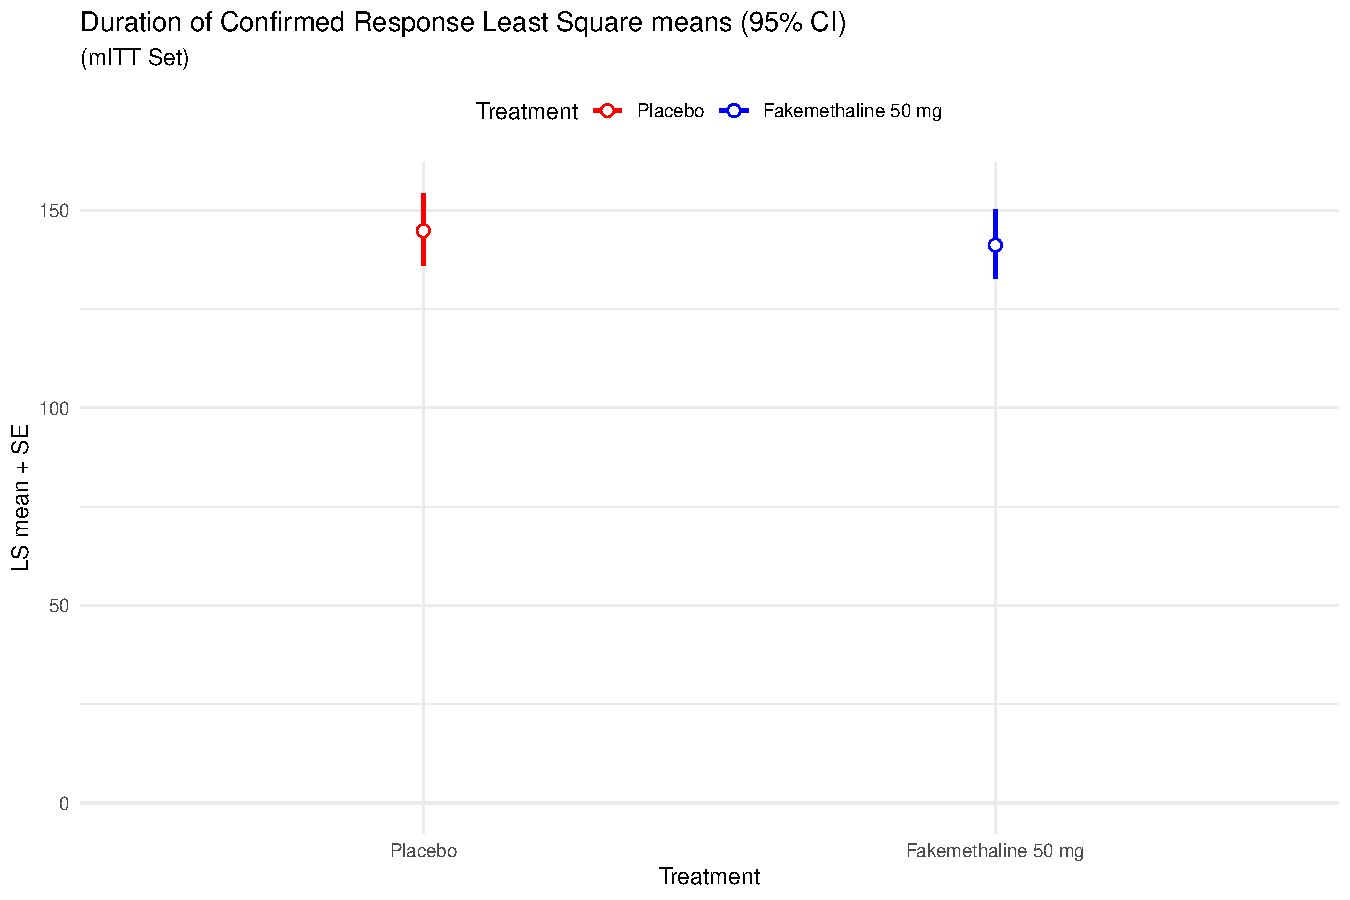
\includegraphics[keepaspectratio]{Negative-Binomial---Efficacy_files/figure-pdf/do the analysis-1.pdf}}
\newpage

\begin{longtable}[]{@{}
  >{\raggedright\arraybackslash}p{(\linewidth - 10\tabcolsep) * \real{0.3562}}
  >{\raggedright\arraybackslash}p{(\linewidth - 10\tabcolsep) * \real{0.0753}}
  >{\raggedright\arraybackslash}p{(\linewidth - 10\tabcolsep) * \real{0.1712}}
  >{\raggedright\arraybackslash}p{(\linewidth - 10\tabcolsep) * \real{0.1712}}
  >{\raggedright\arraybackslash}p{(\linewidth - 10\tabcolsep) * \real{0.1712}}
  >{\raggedright\arraybackslash}p{(\linewidth - 10\tabcolsep) * \real{0.0548}}@{}}
\caption{Annualized Relapse Rate: Parameter = Duration of Confirmed
Response (mITT Population)}\tabularnewline
\toprule\noalign{}
\begin{minipage}[b]{\linewidth}\raggedright
Parameter
\end{minipage} & \begin{minipage}[b]{\linewidth}\raggedright
Statistics
\end{minipage} & \begin{minipage}[b]{\linewidth}\raggedright
Fakemethaline 150 mg
\end{minipage} & \begin{minipage}[b]{\linewidth}\raggedright
Placebo
\end{minipage} & \begin{minipage}[b]{\linewidth}\raggedright
Comparison
\end{minipage} & \begin{minipage}[b]{\linewidth}\raggedright
P-Value
\end{minipage} \\
\midrule\noalign{}
\endfirsthead
\toprule\noalign{}
\begin{minipage}[b]{\linewidth}\raggedright
Parameter
\end{minipage} & \begin{minipage}[b]{\linewidth}\raggedright
Statistics
\end{minipage} & \begin{minipage}[b]{\linewidth}\raggedright
Fakemethaline 150 mg
\end{minipage} & \begin{minipage}[b]{\linewidth}\raggedright
Placebo
\end{minipage} & \begin{minipage}[b]{\linewidth}\raggedright
Comparison
\end{minipage} & \begin{minipage}[b]{\linewidth}\raggedright
P-Value
\end{minipage} \\
\midrule\noalign{}
\endhead
\bottomrule\noalign{}
\endlastfoot
Duration of treatment (years) & n & 132 & 134 & & \\
& Mean (SD) & 2.697 (0.548) & 2.6 (0.612) & & \\
& Median & 3.001 & 3.001 & & \\
& Q1/Q3 & 2.63/3 & 2.14/3 & & \\
& Min/Max & 1.01/3 & 1.06/3 & & \\
& & & & & \\
Duration of Confirmed Response & n & 132 & 134 & & \\
& Mean (SD) & 133.902 (41.365) & 146.908 (38.743) & & \\
& Median & 134.582 & 149.859 & & \\
& Q1/Q3 & 110.86/165.93 & 121/180.82 & & \\
& Min/Max & 16.21/199.85 & 27.98/198.65 & & \\
& & & & & \\
Cumulative treatment time (subject years) & & 355.99 & 348.45 & & \\
Cumulative number of Duration of Confirmed Response & & 17675.04 &
19685.65 & & \\
Raw Annualized Relapse Rate & & 49.65 & 56.49 & & \\
Rate Ratio & & & & 0.879 & \\
Difference & & & & -6.84 & \\
& & & & & \\
Least square means (95\% CI) & & 115.531(82.726, 161.345) &
126.877(90.426, 178.023) & & \\
Difference & & & & -11.347(-22.026, -0.667) & \\
Rate Ratio & & & & 0.911(0.837, 0.984) & 0.0227 \\
\end{longtable}

\newpage

\pandocbounded{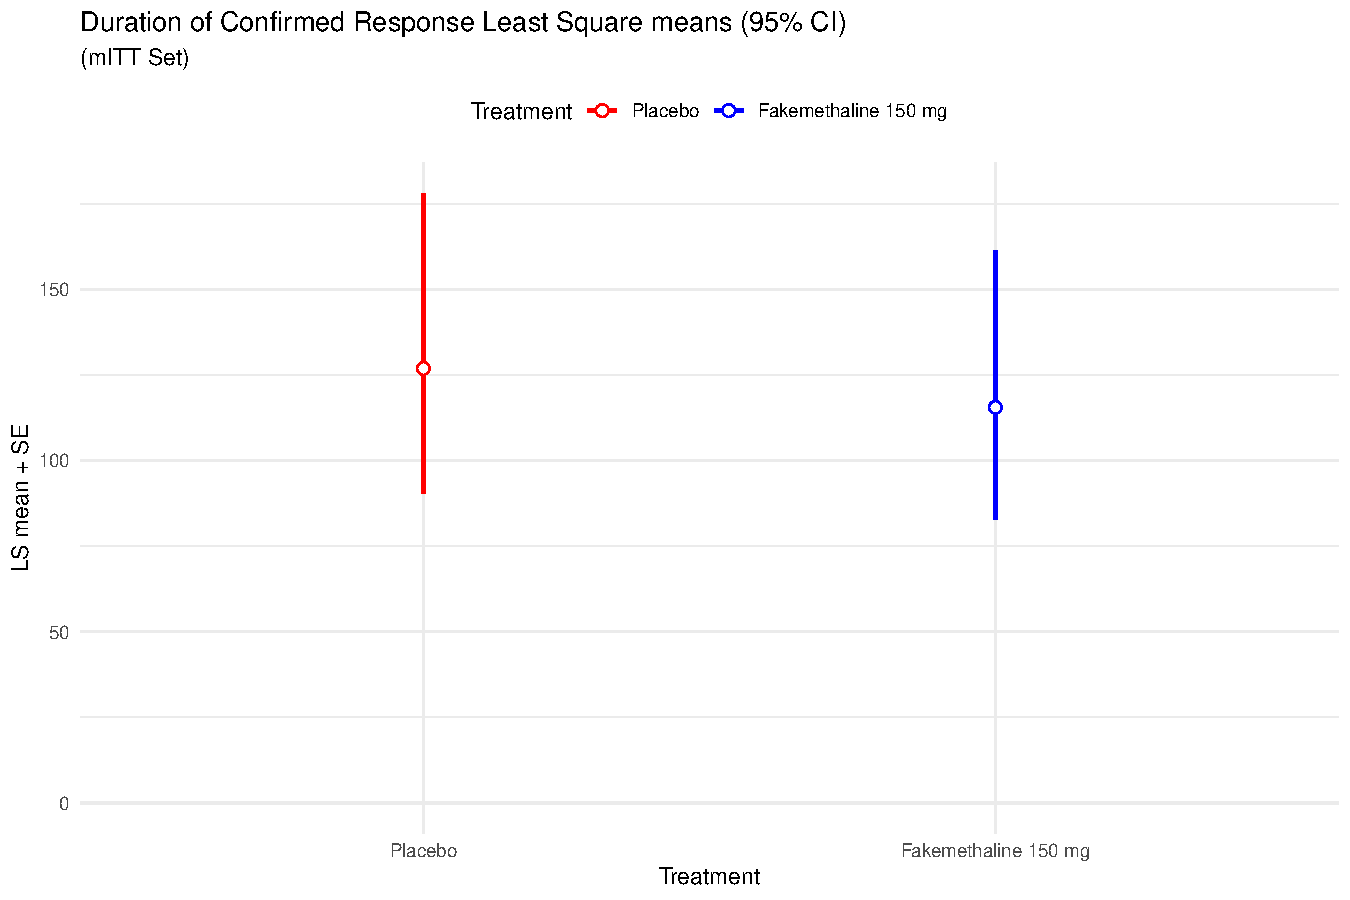
\includegraphics[keepaspectratio]{Negative-Binomial---Efficacy_files/figure-pdf/do the analysis-2.pdf}}
\newpage

\begin{longtable}[]{@{}
  >{\raggedright\arraybackslash}p{(\linewidth - 10\tabcolsep) * \real{0.3281}}
  >{\raggedright\arraybackslash}p{(\linewidth - 10\tabcolsep) * \real{0.0859}}
  >{\raggedright\arraybackslash}p{(\linewidth - 10\tabcolsep) * \real{0.1797}}
  >{\raggedright\arraybackslash}p{(\linewidth - 10\tabcolsep) * \real{0.1719}}
  >{\raggedright\arraybackslash}p{(\linewidth - 10\tabcolsep) * \real{0.1719}}
  >{\raggedright\arraybackslash}p{(\linewidth - 10\tabcolsep) * \real{0.0625}}@{}}
\caption{Annualized Relapse Rate: Parameter = Event Free Survival (mITT
Population)}\tabularnewline
\toprule\noalign{}
\begin{minipage}[b]{\linewidth}\raggedright
Parameter
\end{minipage} & \begin{minipage}[b]{\linewidth}\raggedright
Statistics
\end{minipage} & \begin{minipage}[b]{\linewidth}\raggedright
Fakemethaline 50 mg
\end{minipage} & \begin{minipage}[b]{\linewidth}\raggedright
Placebo
\end{minipage} & \begin{minipage}[b]{\linewidth}\raggedright
Comparison
\end{minipage} & \begin{minipage}[b]{\linewidth}\raggedright
P-Value
\end{minipage} \\
\midrule\noalign{}
\endfirsthead
\toprule\noalign{}
\begin{minipage}[b]{\linewidth}\raggedright
Parameter
\end{minipage} & \begin{minipage}[b]{\linewidth}\raggedright
Statistics
\end{minipage} & \begin{minipage}[b]{\linewidth}\raggedright
Fakemethaline 50 mg
\end{minipage} & \begin{minipage}[b]{\linewidth}\raggedright
Placebo
\end{minipage} & \begin{minipage}[b]{\linewidth}\raggedright
Comparison
\end{minipage} & \begin{minipage}[b]{\linewidth}\raggedright
P-Value
\end{minipage} \\
\midrule\noalign{}
\endhead
\bottomrule\noalign{}
\endlastfoot
Duration of treatment (years) & n & 134 & 134 & & \\
& Mean (SD) & 2.633 (0.571) & 2.6 (0.612) & & \\
& Median & 3.001 & 3.001 & & \\
& Q1/Q3 & 2.36/3 & 2.14/3 & & \\
& Min/Max & 1.08/3 & 1.06/3 & & \\
& & & & & \\
Event Free Survival & n & 134 & 134 & & \\
& Mean (SD) & 55.757 (24.431) & 56.532 (25.9) & & \\
& Median & 55.643 & 55.038 & & \\
& Q1/Q3 & 35.47/75.47 & 34.04/78.82 & & \\
& Min/Max & 15.05/98.16 & 15.67/99.9 & & \\
& & & & & \\
Cumulative treatment time (subject years) & & 352.87 & 348.45 & & \\
Cumulative number of Event Free Survival & & 7471.4 & 7575.32 & & \\
Raw Annualized Relapse Rate & & 21.17 & 21.74 & & \\
Rate Ratio & & & & 0.974 & \\
Difference & & & & -0.569999999999997 & \\
& & & & & \\
Least square means (95\% CI) & & 55.889(50.888, 61.381) & 56.683(51.47,
62.423) & & \\
Difference & & & & -0.794(-7.234, 5.647) & \\
Rate Ratio & & & & 0.986(0.873, 1.099) & 0.809 \\
\end{longtable}

\newpage

\pandocbounded{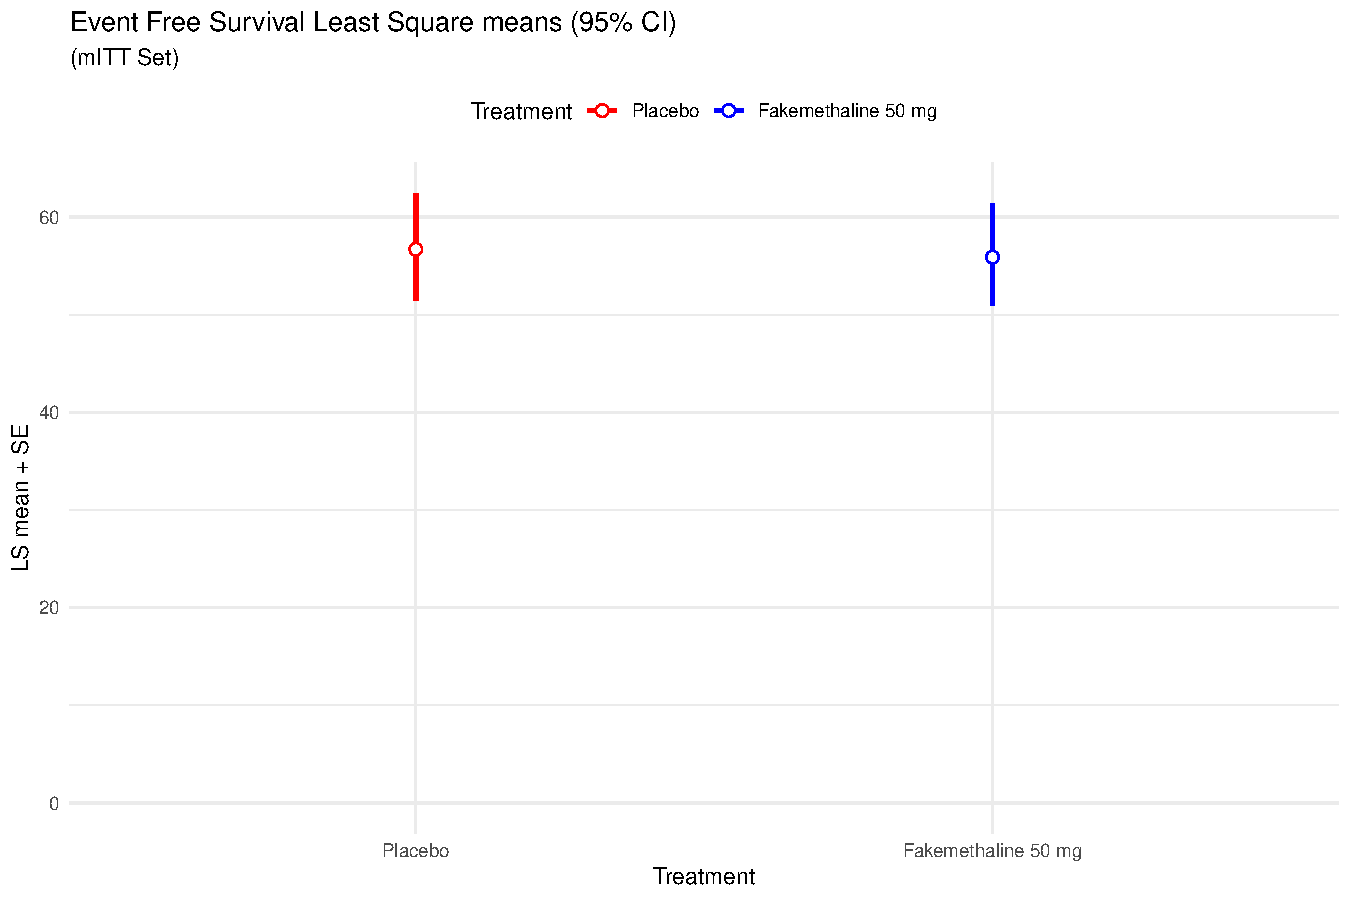
\includegraphics[keepaspectratio]{Negative-Binomial---Efficacy_files/figure-pdf/do the analysis-3.pdf}}
\newpage

\begin{longtable}[]{@{}
  >{\raggedright\arraybackslash}p{(\linewidth - 10\tabcolsep) * \real{0.3281}}
  >{\raggedright\arraybackslash}p{(\linewidth - 10\tabcolsep) * \real{0.0859}}
  >{\raggedright\arraybackslash}p{(\linewidth - 10\tabcolsep) * \real{0.1719}}
  >{\raggedright\arraybackslash}p{(\linewidth - 10\tabcolsep) * \real{0.1797}}
  >{\raggedright\arraybackslash}p{(\linewidth - 10\tabcolsep) * \real{0.1719}}
  >{\raggedright\arraybackslash}p{(\linewidth - 10\tabcolsep) * \real{0.0625}}@{}}
\caption{Annualized Relapse Rate: Parameter = Event Free Survival (mITT
Population)}\tabularnewline
\toprule\noalign{}
\begin{minipage}[b]{\linewidth}\raggedright
Parameter
\end{minipage} & \begin{minipage}[b]{\linewidth}\raggedright
Statistics
\end{minipage} & \begin{minipage}[b]{\linewidth}\raggedright
Fakemethaline 150 mg
\end{minipage} & \begin{minipage}[b]{\linewidth}\raggedright
Placebo
\end{minipage} & \begin{minipage}[b]{\linewidth}\raggedright
Comparison
\end{minipage} & \begin{minipage}[b]{\linewidth}\raggedright
P-Value
\end{minipage} \\
\midrule\noalign{}
\endfirsthead
\toprule\noalign{}
\begin{minipage}[b]{\linewidth}\raggedright
Parameter
\end{minipage} & \begin{minipage}[b]{\linewidth}\raggedright
Statistics
\end{minipage} & \begin{minipage}[b]{\linewidth}\raggedright
Fakemethaline 150 mg
\end{minipage} & \begin{minipage}[b]{\linewidth}\raggedright
Placebo
\end{minipage} & \begin{minipage}[b]{\linewidth}\raggedright
Comparison
\end{minipage} & \begin{minipage}[b]{\linewidth}\raggedright
P-Value
\end{minipage} \\
\midrule\noalign{}
\endhead
\bottomrule\noalign{}
\endlastfoot
Duration of treatment (years) & n & 132 & 134 & & \\
& Mean (SD) & 2.697 (0.548) & 2.6 (0.612) & & \\
& Median & 3.001 & 3.001 & & \\
& Q1/Q3 & 2.63/3 & 2.14/3 & & \\
& Min/Max & 1.01/3 & 1.06/3 & & \\
& & & & & \\
Event Free Survival & n & 132 & 134 & & \\
& Mean (SD) & 54.239 (26.405) & 56.532 (25.9) & & \\
& Median & 52.365 & 55.038 & & \\
& Q1/Q3 & 30.45/78.45 & 34.04/78.82 & & \\
& Min/Max & 15.09/99.33 & 15.67/99.9 & & \\
& & & & & \\
Cumulative treatment time (subject years) & & 355.99 & 348.45 & & \\
Cumulative number of Event Free Survival & & 7159.49 & 7575.32 & & \\
Raw Annualized Relapse Rate & & 20.11 & 21.74 & & \\
Rate Ratio & & & & 0.925 & \\
Difference & & & & -1.63 & \\
& & & & & \\
Least square means (95\% CI) & & 45.52(27.379, 75.683) & 47.214(28.198,
79.053) & & \\
Difference & & & & -1.694(-7.457, 4.069) & \\
Rate Ratio & & & & 0.964(0.847, 1.082) & 0.5567 \\
\end{longtable}

\newpage

\pandocbounded{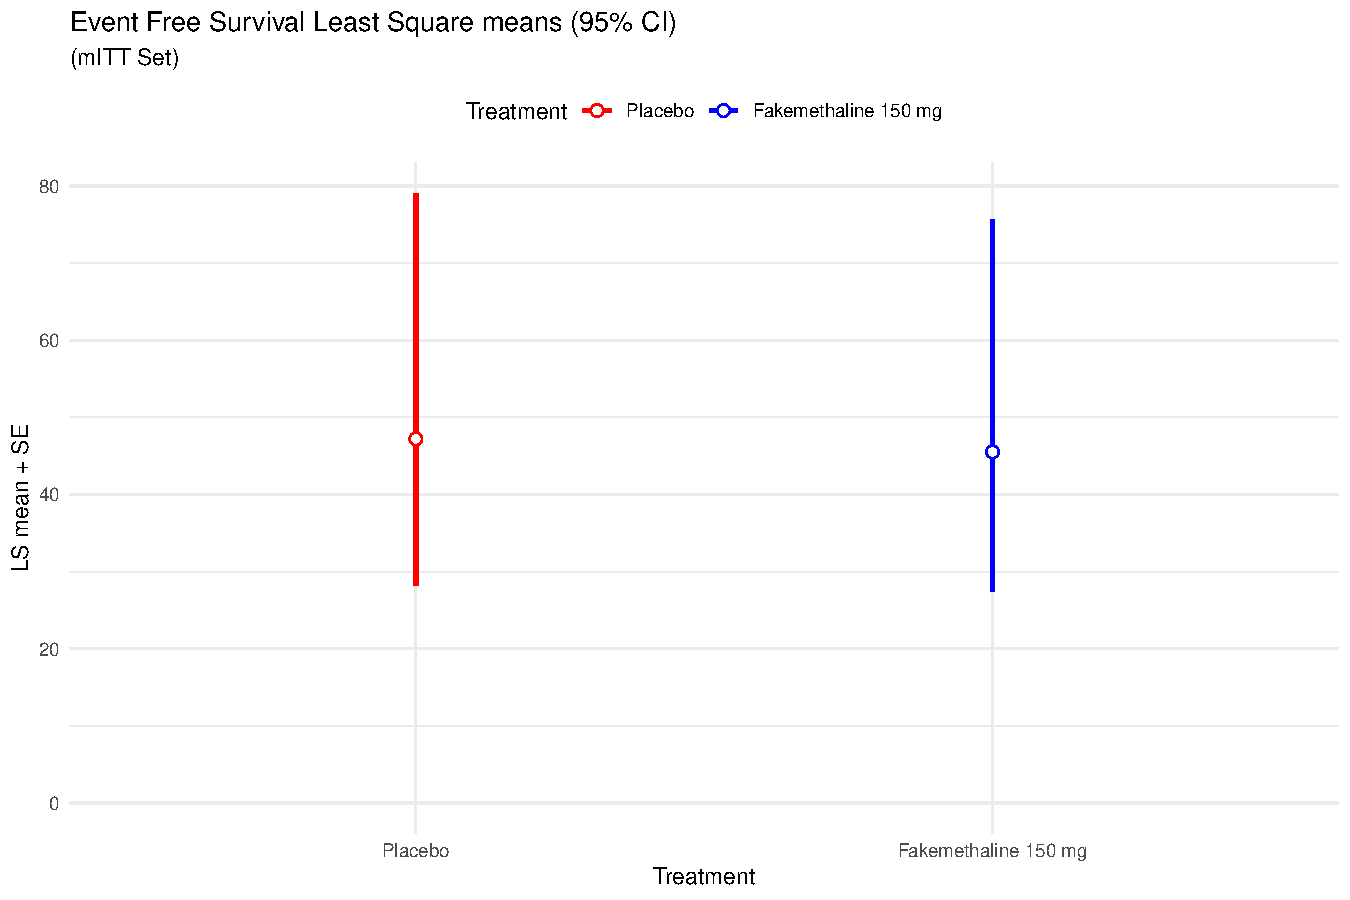
\includegraphics[keepaspectratio]{Negative-Binomial---Efficacy_files/figure-pdf/do the analysis-4.pdf}}
\newpage

\begin{longtable}[]{@{}
  >{\raggedright\arraybackslash}p{(\linewidth - 10\tabcolsep) * \real{0.3088}}
  >{\raggedright\arraybackslash}p{(\linewidth - 10\tabcolsep) * \real{0.0809}}
  >{\raggedright\arraybackslash}p{(\linewidth - 10\tabcolsep) * \real{0.1912}}
  >{\raggedright\arraybackslash}p{(\linewidth - 10\tabcolsep) * \real{0.1912}}
  >{\raggedright\arraybackslash}p{(\linewidth - 10\tabcolsep) * \real{0.1691}}
  >{\raggedright\arraybackslash}p{(\linewidth - 10\tabcolsep) * \real{0.0588}}@{}}
\caption{Annualized Relapse Rate: Parameter = Overall Survival (mITT
Population)}\tabularnewline
\toprule\noalign{}
\begin{minipage}[b]{\linewidth}\raggedright
Parameter
\end{minipage} & \begin{minipage}[b]{\linewidth}\raggedright
Statistics
\end{minipage} & \begin{minipage}[b]{\linewidth}\raggedright
Fakemethaline 50 mg
\end{minipage} & \begin{minipage}[b]{\linewidth}\raggedright
Placebo
\end{minipage} & \begin{minipage}[b]{\linewidth}\raggedright
Comparison
\end{minipage} & \begin{minipage}[b]{\linewidth}\raggedright
P-Value
\end{minipage} \\
\midrule\noalign{}
\endfirsthead
\toprule\noalign{}
\begin{minipage}[b]{\linewidth}\raggedright
Parameter
\end{minipage} & \begin{minipage}[b]{\linewidth}\raggedright
Statistics
\end{minipage} & \begin{minipage}[b]{\linewidth}\raggedright
Fakemethaline 50 mg
\end{minipage} & \begin{minipage}[b]{\linewidth}\raggedright
Placebo
\end{minipage} & \begin{minipage}[b]{\linewidth}\raggedright
Comparison
\end{minipage} & \begin{minipage}[b]{\linewidth}\raggedright
P-Value
\end{minipage} \\
\midrule\noalign{}
\endhead
\bottomrule\noalign{}
\endlastfoot
Duration of treatment (years) & n & 134 & 134 & & \\
& Mean (SD) & 2.633 (0.571) & 2.6 (0.612) & & \\
& Median & 3.001 & 3.001 & & \\
& Q1/Q3 & 2.36/3 & 2.14/3 & & \\
& Min/Max & 1.08/3 & 1.06/3 & & \\
& & & & & \\
Overall Survival & n & 134 & 134 & & \\
& Mean (SD) & 292.725 (135.173) & 290.311 (129.9) & & \\
& Median & 309.611 & 316.349 & & \\
& Q1/Q3 & 169.18/408.97 & 173.32/388.9 & & \\
& Min/Max & 15.05/499.27 & 27.98/495.23 & & \\
& & & & & \\
Cumulative treatment time (subject years) & & 352.87 & 348.45 & & \\
Cumulative number of Overall Survival & & 39225.16 & 38901.68 & & \\
Raw Annualized Relapse Rate & & 111.16 & 111.64 & & \\
Rate Ratio & & & & 0.996 & \\
Difference & & & & -0.480000000000004 & \\
& & & & & \\
Least square means (95\% CI) & & 292.926(263.217, 325.989) &
291.269(260.904, 325.168) & & \\
Difference & & & & 1.657(-36.459, 39.773) & \\
Rate Ratio & & & & 1.006(0.874, 1.137) & 0.9321 \\
\end{longtable}

\newpage

\pandocbounded{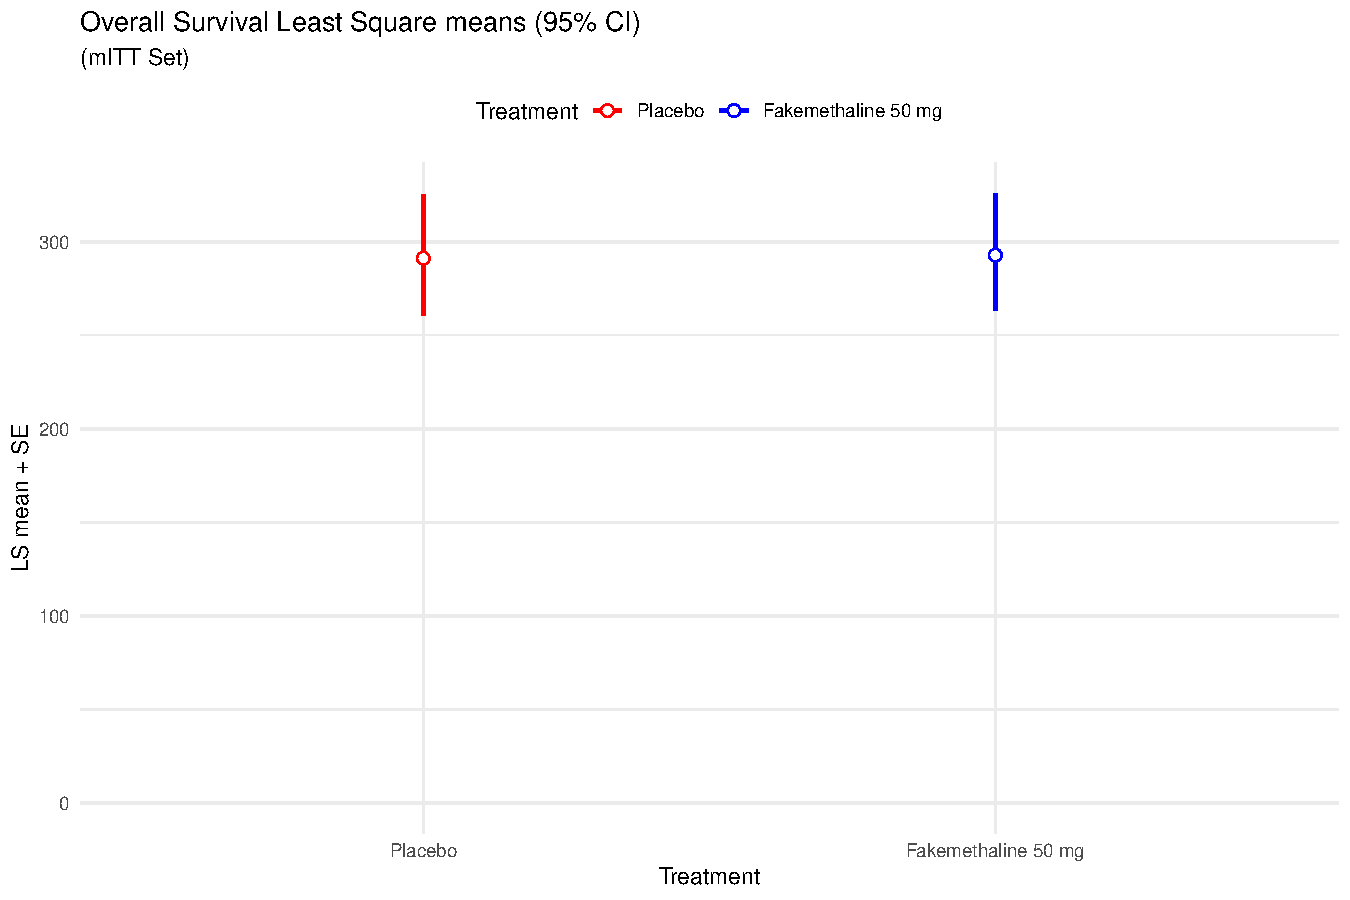
\includegraphics[keepaspectratio]{Negative-Binomial---Efficacy_files/figure-pdf/do the analysis-5.pdf}}
\newpage

\begin{longtable}[]{@{}
  >{\raggedright\arraybackslash}p{(\linewidth - 10\tabcolsep) * \real{0.3043}}
  >{\raggedright\arraybackslash}p{(\linewidth - 10\tabcolsep) * \real{0.0797}}
  >{\raggedright\arraybackslash}p{(\linewidth - 10\tabcolsep) * \real{0.1884}}
  >{\raggedright\arraybackslash}p{(\linewidth - 10\tabcolsep) * \real{0.1884}}
  >{\raggedright\arraybackslash}p{(\linewidth - 10\tabcolsep) * \real{0.1812}}
  >{\raggedright\arraybackslash}p{(\linewidth - 10\tabcolsep) * \real{0.0580}}@{}}
\caption{Annualized Relapse Rate: Parameter = Overall Survival (mITT
Population)}\tabularnewline
\toprule\noalign{}
\begin{minipage}[b]{\linewidth}\raggedright
Parameter
\end{minipage} & \begin{minipage}[b]{\linewidth}\raggedright
Statistics
\end{minipage} & \begin{minipage}[b]{\linewidth}\raggedright
Fakemethaline 150 mg
\end{minipage} & \begin{minipage}[b]{\linewidth}\raggedright
Placebo
\end{minipage} & \begin{minipage}[b]{\linewidth}\raggedright
Comparison
\end{minipage} & \begin{minipage}[b]{\linewidth}\raggedright
P-Value
\end{minipage} \\
\midrule\noalign{}
\endfirsthead
\toprule\noalign{}
\begin{minipage}[b]{\linewidth}\raggedright
Parameter
\end{minipage} & \begin{minipage}[b]{\linewidth}\raggedright
Statistics
\end{minipage} & \begin{minipage}[b]{\linewidth}\raggedright
Fakemethaline 150 mg
\end{minipage} & \begin{minipage}[b]{\linewidth}\raggedright
Placebo
\end{minipage} & \begin{minipage}[b]{\linewidth}\raggedright
Comparison
\end{minipage} & \begin{minipage}[b]{\linewidth}\raggedright
P-Value
\end{minipage} \\
\midrule\noalign{}
\endhead
\bottomrule\noalign{}
\endlastfoot
Duration of treatment (years) & n & 132 & 134 & & \\
& Mean (SD) & 2.697 (0.548) & 2.6 (0.612) & & \\
& Median & 3.001 & 3.001 & & \\
& Q1/Q3 & 2.63/3 & 2.14/3 & & \\
& Min/Max & 1.01/3 & 1.06/3 & & \\
& & & & & \\
Overall Survival & n & 132 & 134 & & \\
& Mean (SD) & 270.94 (135.875) & 290.311 (129.9) & & \\
& Median & 286.629 & 316.349 & & \\
& Q1/Q3 & 154.95/387.42 & 173.32/388.9 & & \\
& Min/Max & 16.21/495.71 & 27.98/495.23 & & \\
& & & & & \\
Cumulative treatment time (subject years) & & 355.99 & 348.45 & & \\
Cumulative number of Overall Survival & & 35764.1 & 38901.68 & & \\
Raw Annualized Relapse Rate & & 100.46 & 111.64 & & \\
Rate Ratio & & & & 0.9 & \\
Difference & & & & -11.18 & \\
& & & & & \\
Least square means (95\% CI) & & 248.903(141.912, 436.556) &
269.156(152.225, 475.905) & & \\
Difference & & & & -20.253(-58.173, 17.667) & \\
Rate Ratio & & & & 0.925(0.798, 1.052) & 0.2633 \\
\end{longtable}

\newpage

\pandocbounded{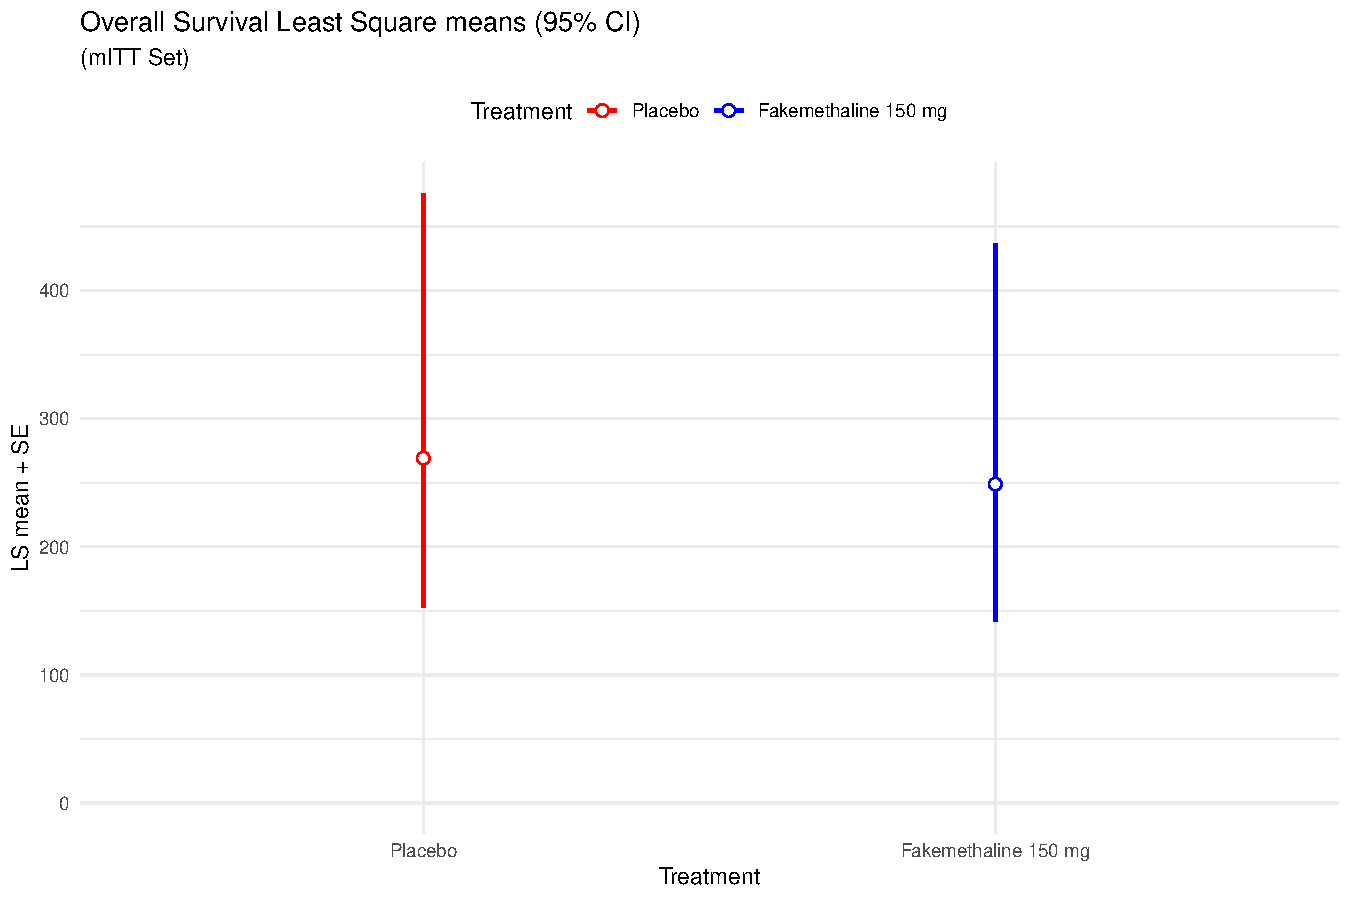
\includegraphics[keepaspectratio]{Negative-Binomial---Efficacy_files/figure-pdf/do the analysis-6.pdf}}
\newpage

\begin{longtable}[]{@{}
  >{\raggedright\arraybackslash}p{(\linewidth - 10\tabcolsep) * \real{0.3357}}
  >{\raggedright\arraybackslash}p{(\linewidth - 10\tabcolsep) * \real{0.0786}}
  >{\raggedright\arraybackslash}p{(\linewidth - 10\tabcolsep) * \real{0.1786}}
  >{\raggedright\arraybackslash}p{(\linewidth - 10\tabcolsep) * \real{0.1857}}
  >{\raggedright\arraybackslash}p{(\linewidth - 10\tabcolsep) * \real{0.1643}}
  >{\raggedright\arraybackslash}p{(\linewidth - 10\tabcolsep) * \real{0.0571}}@{}}
\caption{Annualized Relapse Rate: Parameter = Progression Free Survival
(mITT Population)}\tabularnewline
\toprule\noalign{}
\begin{minipage}[b]{\linewidth}\raggedright
Parameter
\end{minipage} & \begin{minipage}[b]{\linewidth}\raggedright
Statistics
\end{minipage} & \begin{minipage}[b]{\linewidth}\raggedright
Fakemethaline 50 mg
\end{minipage} & \begin{minipage}[b]{\linewidth}\raggedright
Placebo
\end{minipage} & \begin{minipage}[b]{\linewidth}\raggedright
Comparison
\end{minipage} & \begin{minipage}[b]{\linewidth}\raggedright
P-Value
\end{minipage} \\
\midrule\noalign{}
\endfirsthead
\toprule\noalign{}
\begin{minipage}[b]{\linewidth}\raggedright
Parameter
\end{minipage} & \begin{minipage}[b]{\linewidth}\raggedright
Statistics
\end{minipage} & \begin{minipage}[b]{\linewidth}\raggedright
Fakemethaline 50 mg
\end{minipage} & \begin{minipage}[b]{\linewidth}\raggedright
Placebo
\end{minipage} & \begin{minipage}[b]{\linewidth}\raggedright
Comparison
\end{minipage} & \begin{minipage}[b]{\linewidth}\raggedright
P-Value
\end{minipage} \\
\midrule\noalign{}
\endhead
\bottomrule\noalign{}
\endlastfoot
Duration of treatment (years) & n & 134 & 134 & & \\
& Mean (SD) & 2.633 (0.571) & 2.6 (0.612) & & \\
& Median & 3.001 & 3.001 & & \\
& Q1/Q3 & 2.36/3 & 2.14/3 & & \\
& Min/Max & 1.08/3 & 1.06/3 & & \\
& & & & & \\
Progression Free Survival & n & 134 & 134 & & \\
& Mean (SD) & 211.946 (71.098) & 210.394 (67.746) & & \\
& Median & 230.33 & 225.776 & & \\
& Q1/Q3 & 169.18/268.36 & 173.32/264.61 & & \\
& Min/Max & 15.05/299.48 & 27.98/299.53 & & \\
& & & & & \\
Cumulative treatment time (subject years) & & 352.87 & 348.45 & & \\
Cumulative number of Progression Free Survival & & 28400.7 & 28192.83 &
& \\
Raw Annualized Relapse Rate & & 80.48 & 80.91 & & \\
Rate Ratio & & & & 0.995 & \\
Difference & & & & -0.429999999999993 & \\
& & & & & \\
Least square means (95\% CI) & & 210.198(194.134, 227.59) &
209.489(193.027, 227.355) & & \\
Difference & & & & 0.709(-19.645, 21.063) & \\
Rate Ratio & & & & 1.003(0.906, 1.101) & 0.9456 \\
\end{longtable}

\newpage

\pandocbounded{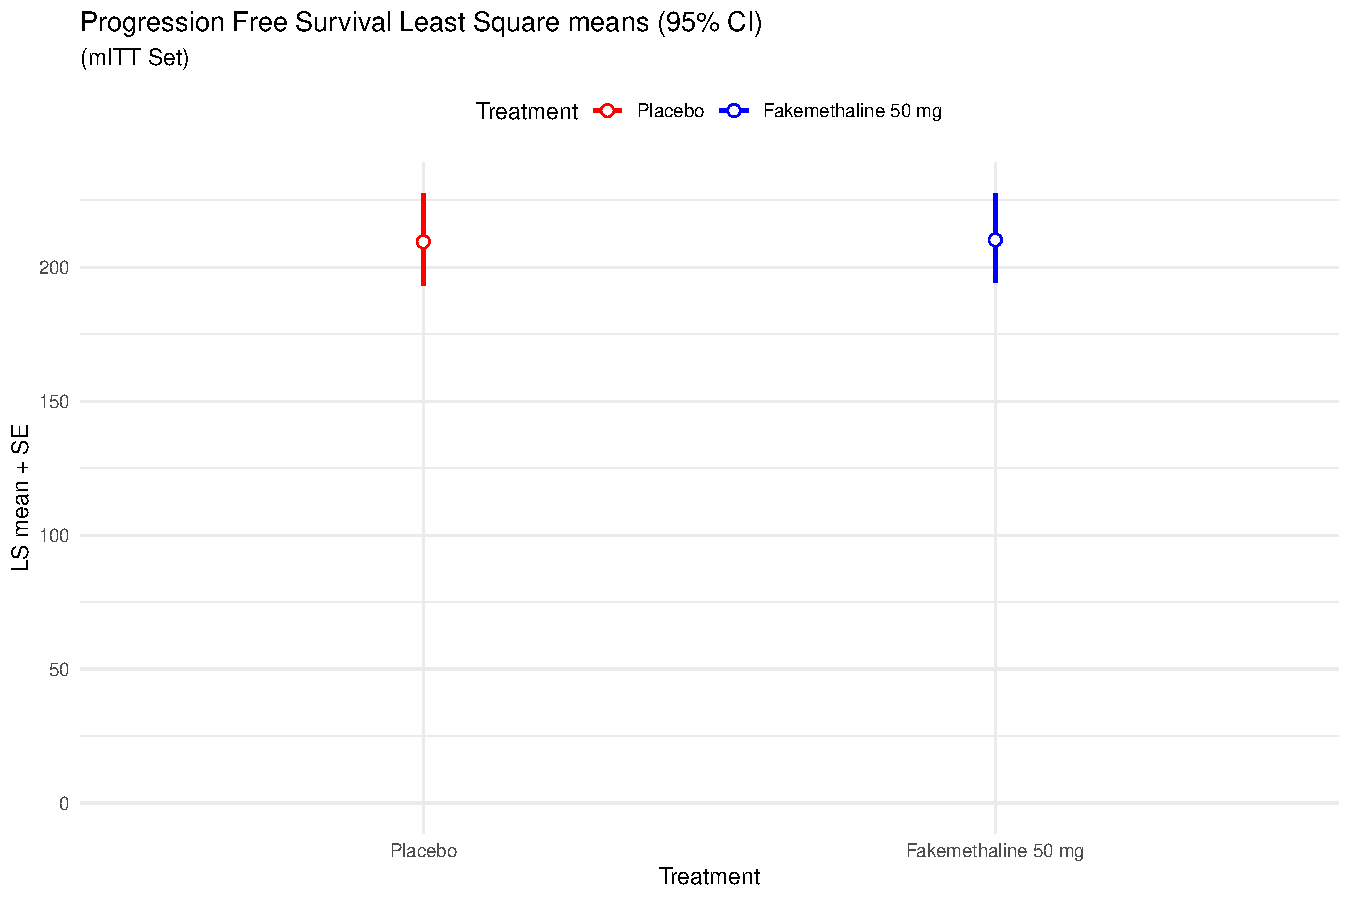
\includegraphics[keepaspectratio]{Negative-Binomial---Efficacy_files/figure-pdf/do the analysis-7.pdf}}
\newpage

\begin{longtable}[]{@{}
  >{\raggedright\arraybackslash}p{(\linewidth - 10\tabcolsep) * \real{0.3333}}
  >{\raggedright\arraybackslash}p{(\linewidth - 10\tabcolsep) * \real{0.0780}}
  >{\raggedright\arraybackslash}p{(\linewidth - 10\tabcolsep) * \real{0.1844}}
  >{\raggedright\arraybackslash}p{(\linewidth - 10\tabcolsep) * \real{0.1702}}
  >{\raggedright\arraybackslash}p{(\linewidth - 10\tabcolsep) * \real{0.1773}}
  >{\raggedright\arraybackslash}p{(\linewidth - 10\tabcolsep) * \real{0.0567}}@{}}
\caption{Annualized Relapse Rate: Parameter = Progression Free Survival
(mITT Population)}\tabularnewline
\toprule\noalign{}
\begin{minipage}[b]{\linewidth}\raggedright
Parameter
\end{minipage} & \begin{minipage}[b]{\linewidth}\raggedright
Statistics
\end{minipage} & \begin{minipage}[b]{\linewidth}\raggedright
Fakemethaline 150 mg
\end{minipage} & \begin{minipage}[b]{\linewidth}\raggedright
Placebo
\end{minipage} & \begin{minipage}[b]{\linewidth}\raggedright
Comparison
\end{minipage} & \begin{minipage}[b]{\linewidth}\raggedright
P-Value
\end{minipage} \\
\midrule\noalign{}
\endfirsthead
\toprule\noalign{}
\begin{minipage}[b]{\linewidth}\raggedright
Parameter
\end{minipage} & \begin{minipage}[b]{\linewidth}\raggedright
Statistics
\end{minipage} & \begin{minipage}[b]{\linewidth}\raggedright
Fakemethaline 150 mg
\end{minipage} & \begin{minipage}[b]{\linewidth}\raggedright
Placebo
\end{minipage} & \begin{minipage}[b]{\linewidth}\raggedright
Comparison
\end{minipage} & \begin{minipage}[b]{\linewidth}\raggedright
P-Value
\end{minipage} \\
\midrule\noalign{}
\endhead
\bottomrule\noalign{}
\endlastfoot
Duration of treatment (years) & n & 132 & 134 & & \\
& Mean (SD) & 2.697 (0.548) & 2.6 (0.612) & & \\
& Median & 3.001 & 3.001 & & \\
& Q1/Q3 & 2.63/3 & 2.14/3 & & \\
& Min/Max & 1.01/3 & 1.06/3 & & \\
& & & & & \\
Progression Free Survival & n & 132 & 134 & & \\
& Mean (SD) & 201.179 (73.689) & 210.394 (67.746) & & \\
& Median & 220.978 & 225.776 & & \\
& Q1/Q3 & 154.95/256.17 & 173.32/264.61 & & \\
& Min/Max & 16.21/297.87 & 27.98/299.53 & & \\
& & & & & \\
Cumulative treatment time (subject years) & & 355.99 & 348.45 & & \\
Cumulative number of Progression Free Survival & & 26555.6 & 28192.83 &
& \\
Raw Annualized Relapse Rate & & 74.6 & 80.91 & & \\
Rate Ratio & & & & 0.922 & \\
Difference & & & & -6.31 & \\
& & & & & \\
Least square means (95\% CI) & & 215.707(141.212, 329.501) &
228.119(148.426, 350.6) & & \\
Difference & & & & -12.412(-36.309, 11.485) & \\
Rate Ratio & & & & 0.946(0.848, 1.044) & 0.2901 \\
\end{longtable}

\newpage

\pandocbounded{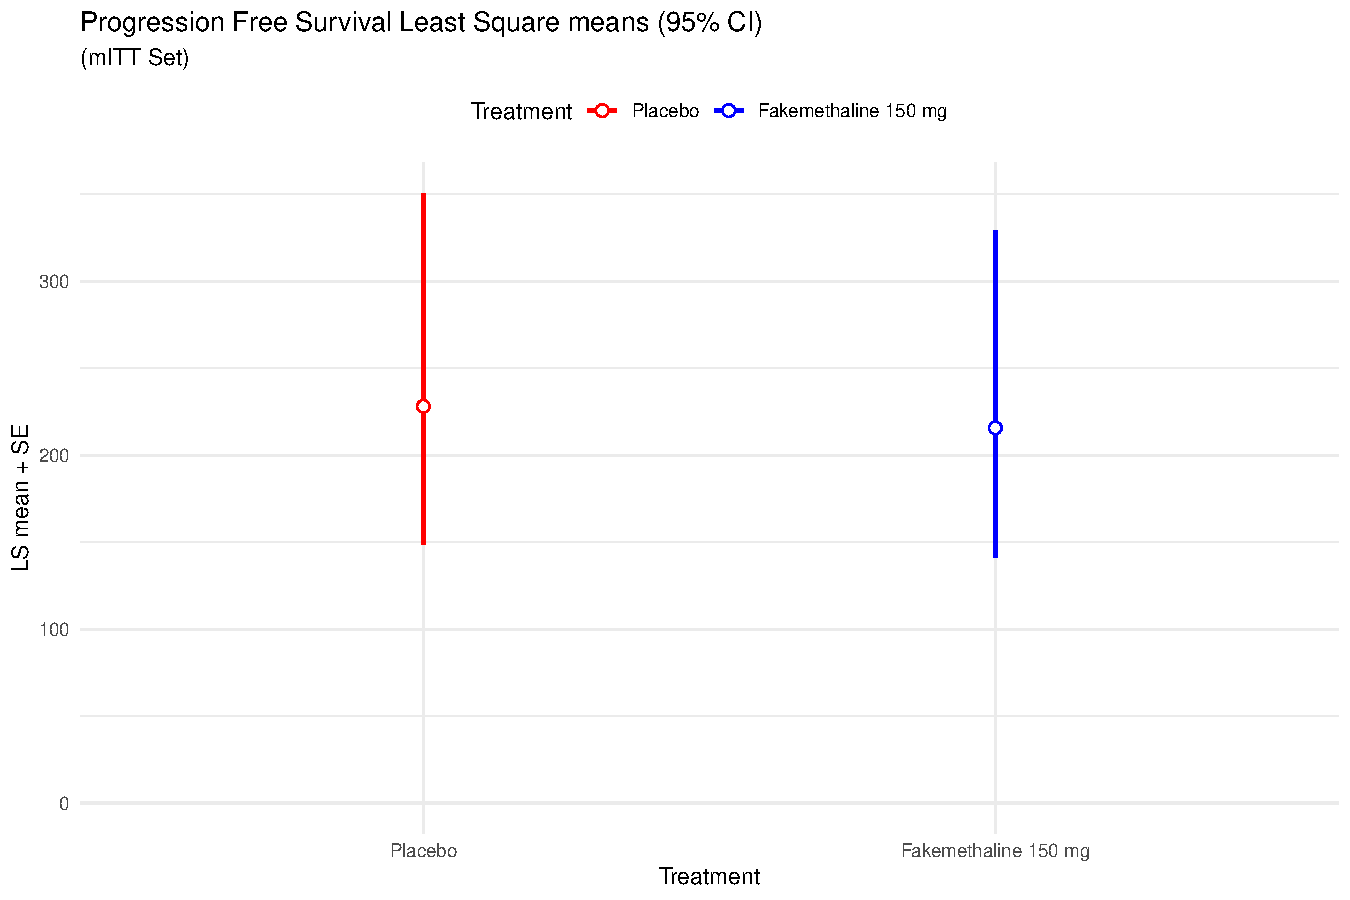
\includegraphics[keepaspectratio]{Negative-Binomial---Efficacy_files/figure-pdf/do the analysis-8.pdf}}
\newpage

\begin{longtable}[]{@{}
  >{\raggedright\arraybackslash}p{(\linewidth - 10\tabcolsep) * \real{0.3893}}
  >{\raggedright\arraybackslash}p{(\linewidth - 10\tabcolsep) * \real{0.0840}}
  >{\raggedright\arraybackslash}p{(\linewidth - 10\tabcolsep) * \real{0.1527}}
  >{\raggedright\arraybackslash}p{(\linewidth - 10\tabcolsep) * \real{0.1527}}
  >{\raggedright\arraybackslash}p{(\linewidth - 10\tabcolsep) * \real{0.1603}}
  >{\raggedright\arraybackslash}p{(\linewidth - 10\tabcolsep) * \real{0.0611}}@{}}
\caption{Annualized Relapse Rate: Parameter = Total Number of
Exacerbations (mITT Population)}\tabularnewline
\toprule\noalign{}
\begin{minipage}[b]{\linewidth}\raggedright
Parameter
\end{minipage} & \begin{minipage}[b]{\linewidth}\raggedright
Statistics
\end{minipage} & \begin{minipage}[b]{\linewidth}\raggedright
Fakemethaline 50 mg
\end{minipage} & \begin{minipage}[b]{\linewidth}\raggedright
Placebo
\end{minipage} & \begin{minipage}[b]{\linewidth}\raggedright
Comparison
\end{minipage} & \begin{minipage}[b]{\linewidth}\raggedright
P-Value
\end{minipage} \\
\midrule\noalign{}
\endfirsthead
\toprule\noalign{}
\begin{minipage}[b]{\linewidth}\raggedright
Parameter
\end{minipage} & \begin{minipage}[b]{\linewidth}\raggedright
Statistics
\end{minipage} & \begin{minipage}[b]{\linewidth}\raggedright
Fakemethaline 50 mg
\end{minipage} & \begin{minipage}[b]{\linewidth}\raggedright
Placebo
\end{minipage} & \begin{minipage}[b]{\linewidth}\raggedright
Comparison
\end{minipage} & \begin{minipage}[b]{\linewidth}\raggedright
P-Value
\end{minipage} \\
\midrule\noalign{}
\endhead
\bottomrule\noalign{}
\endlastfoot
Duration of treatment (years) & n & 134 & 134 & & \\
& Mean (SD) & 2.633 (0.571) & 2.6 (0.612) & & \\
& Median & 3.001 & 3.001 & & \\
& Q1/Q3 & 2.36/3 & 2.14/3 & & \\
& Min/Max & 1.08/3 & 1.06/3 & & \\
& & & & & \\
Total Number of Exacerbations & n & 134 & 134 & & \\
& Mean (SD) & 2.843 (1.703) & 2.776 (1.894) & & \\
& Median & 2 & 2 & & \\
& Q1/Q3 & 2/4 & 1/4 & & \\
& Min/Max & 0/8 & 0/9 & & \\
& & & & & \\
Cumulative treatment time (subject years) & & 352.87 & 348.45 & & \\
Cumulative number of Total Number of Exacerbations & & 381 & 372 & & \\
Raw Annualized Relapse Rate & & 1.08 & 1.07 & & \\
Rate Ratio & & & & 1.009 & \\
Difference & & & & 0.01 & \\
& & & & & \\
Least square means (95\% CI) & & 2.763(2.435, 3.134) & 2.684(2.355,
3.059) & & \\
Difference & & & & 0.078(-0.337, 0.494) & \\
Rate Ratio & & & & 1.029(0.872, 1.186) & 0.7121 \\
\end{longtable}

\newpage

\pandocbounded{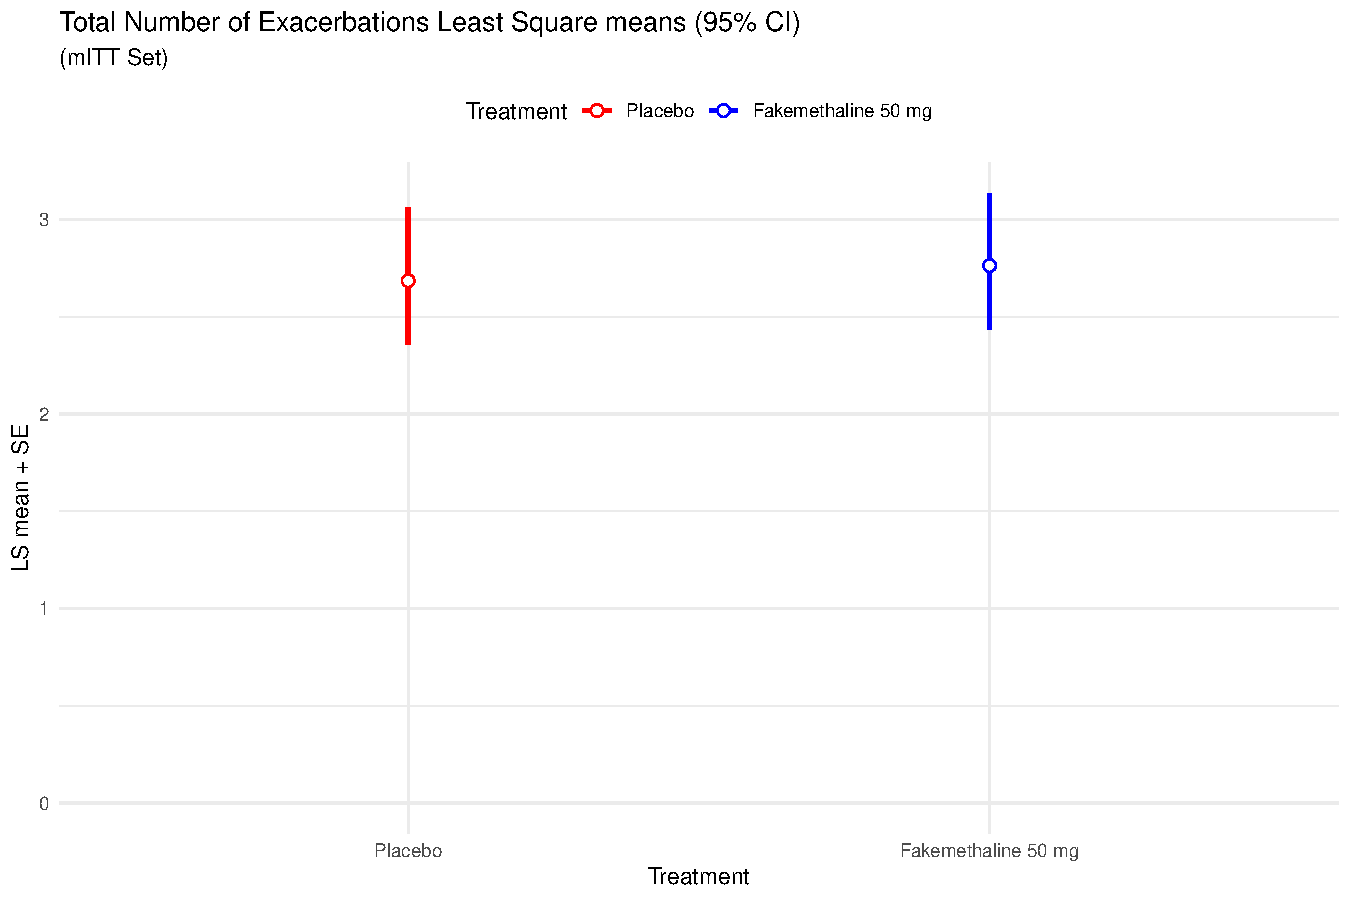
\includegraphics[keepaspectratio]{Negative-Binomial---Efficacy_files/figure-pdf/do the analysis-9.pdf}}
\newpage

\begin{longtable}[]{@{}
  >{\raggedright\arraybackslash}p{(\linewidth - 10\tabcolsep) * \real{0.3893}}
  >{\raggedright\arraybackslash}p{(\linewidth - 10\tabcolsep) * \real{0.0840}}
  >{\raggedright\arraybackslash}p{(\linewidth - 10\tabcolsep) * \real{0.1603}}
  >{\raggedright\arraybackslash}p{(\linewidth - 10\tabcolsep) * \real{0.1527}}
  >{\raggedright\arraybackslash}p{(\linewidth - 10\tabcolsep) * \real{0.1527}}
  >{\raggedright\arraybackslash}p{(\linewidth - 10\tabcolsep) * \real{0.0611}}@{}}
\caption{Annualized Relapse Rate: Parameter = Total Number of
Exacerbations (mITT Population)}\tabularnewline
\toprule\noalign{}
\begin{minipage}[b]{\linewidth}\raggedright
Parameter
\end{minipage} & \begin{minipage}[b]{\linewidth}\raggedright
Statistics
\end{minipage} & \begin{minipage}[b]{\linewidth}\raggedright
Fakemethaline 150 mg
\end{minipage} & \begin{minipage}[b]{\linewidth}\raggedright
Placebo
\end{minipage} & \begin{minipage}[b]{\linewidth}\raggedright
Comparison
\end{minipage} & \begin{minipage}[b]{\linewidth}\raggedright
P-Value
\end{minipage} \\
\midrule\noalign{}
\endfirsthead
\toprule\noalign{}
\begin{minipage}[b]{\linewidth}\raggedright
Parameter
\end{minipage} & \begin{minipage}[b]{\linewidth}\raggedright
Statistics
\end{minipage} & \begin{minipage}[b]{\linewidth}\raggedright
Fakemethaline 150 mg
\end{minipage} & \begin{minipage}[b]{\linewidth}\raggedright
Placebo
\end{minipage} & \begin{minipage}[b]{\linewidth}\raggedright
Comparison
\end{minipage} & \begin{minipage}[b]{\linewidth}\raggedright
P-Value
\end{minipage} \\
\midrule\noalign{}
\endhead
\bottomrule\noalign{}
\endlastfoot
Duration of treatment (years) & n & 132 & 134 & & \\
& Mean (SD) & 2.697 (0.548) & 2.6 (0.612) & & \\
& Median & 3.001 & 3.001 & & \\
& Q1/Q3 & 2.63/3 & 2.14/3 & & \\
& Min/Max & 1.01/3 & 1.06/3 & & \\
& & & & & \\
Total Number of Exacerbations & n & 132 & 134 & & \\
& Mean (SD) & 2.985 (1.752) & 2.776 (1.894) & & \\
& Median & 3 & 2 & & \\
& Q1/Q3 & 2/4 & 1/4 & & \\
& Min/Max & 0/8 & 0/9 & & \\
& & & & & \\
Cumulative treatment time (subject years) & & 355.99 & 348.45 & & \\
Cumulative number of Total Number of Exacerbations & & 394 & 372 & & \\
Raw Annualized Relapse Rate & & 1.11 & 1.07 & & \\
Rate Ratio & & & & 1.037 & \\
Difference & & & & 0.04 & \\
& & & & & \\
Least square means (95\% CI) & & 2.335(1.121, 4.861) & 2.166(1.032,
4.545) & & \\
Difference & & & & 0.169(-0.19, 0.527) & \\
Rate Ratio & & & & 1.078(0.913, 1.242) & 0.3352 \\
\end{longtable}

\newpage

\pandocbounded{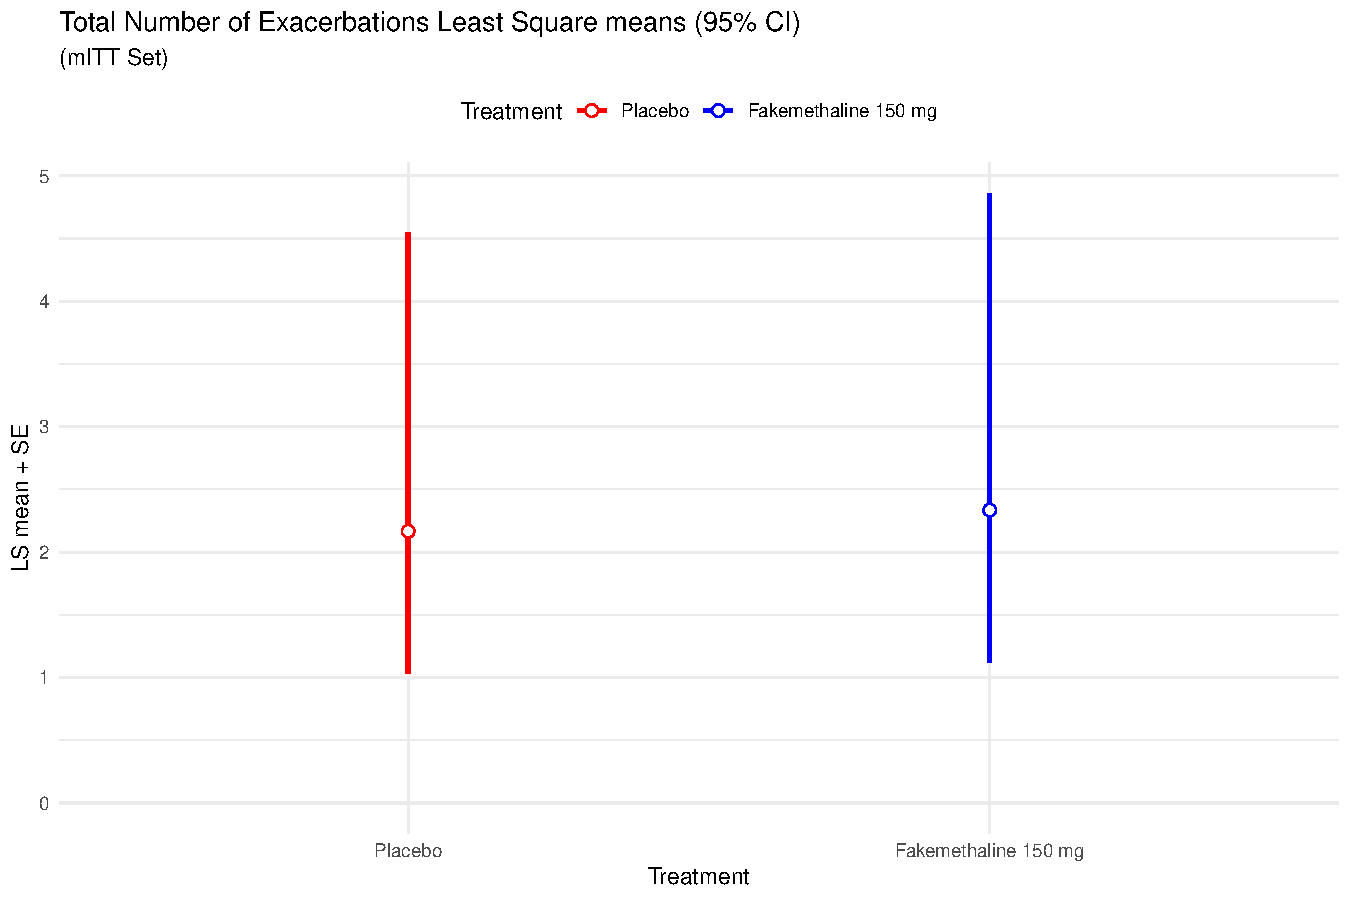
\includegraphics[keepaspectratio]{Negative-Binomial---Efficacy_files/figure-pdf/do the analysis-10.pdf}}
\newpage




\end{document}
